\documentclass[a4paper,11pt]{article}
\usepackage{tabularx} % extra features for tabular environment
\usepackage{amsmath}  % improve math presentation
\usepackage{graphicx} % takes care of graphic including machinery
\usepackage[margin=1in,letterpaper]{geometry} % decreases margins
\usepackage{cite} % takes care of citations
\usepackage[final]{hyperref} % adds hyper links inside the generated pdf file
\hypersetup{
	colorlinks=true,       % false: boxed links; true: colored links
	linkcolor=blue,        % color of internal links
	citecolor=blue,        % color of links to bibliography
	filecolor=magenta,     % color of file links
	urlcolor=blue         
}
\topmargin 0.0cm
\oddsidemargin 0.2cm
\textwidth 16cm 
\textheight 21cm
\footskip 1.0cm

% \usepackage{blindtext}
% \usepackage{biblatex}
% \addbibresource{main.bib}

% \usepackage[nottoc]{tocbibind}

\usepackage[ruled,vlined,linesnumbered,noend]{algorithm2e}
% \usepackage{algorithm}

%++++++++++++++++++++++++++++++++++++++++


\begin{document}

\title{RL Autonomous Guidance of Human Controlled Vehicle}
\author{Matan Weksler, \  Ido Glanz
}
\date{\today}
\maketitle


\section{Introduction}

We choose to tackle the task of Human-Robot Interaction (HRI) in the form of robotic guidance, and namely the task of an autonomous drone needing to guide a human agent through a simulated 3D grid-world environment. The task as we perceive it is the need for the robot agent to learn the human control constraints (such as latency, line-of-sight to the robot, manoeuvrability etc.) as to allow the human to properly follow it along the path yet do it in minimal time. In other words, the drone will need to learn to optimize it’s flight speed (including reaching a complete stop) so a human-controlled car can follow it along a path. The drone will monitor their relative state and decide on it’s action at a 1Hz loop, concluding a successful episode if they both reach the goal within a reasonable lag.

\begin{figure}[!h]
    \centering
    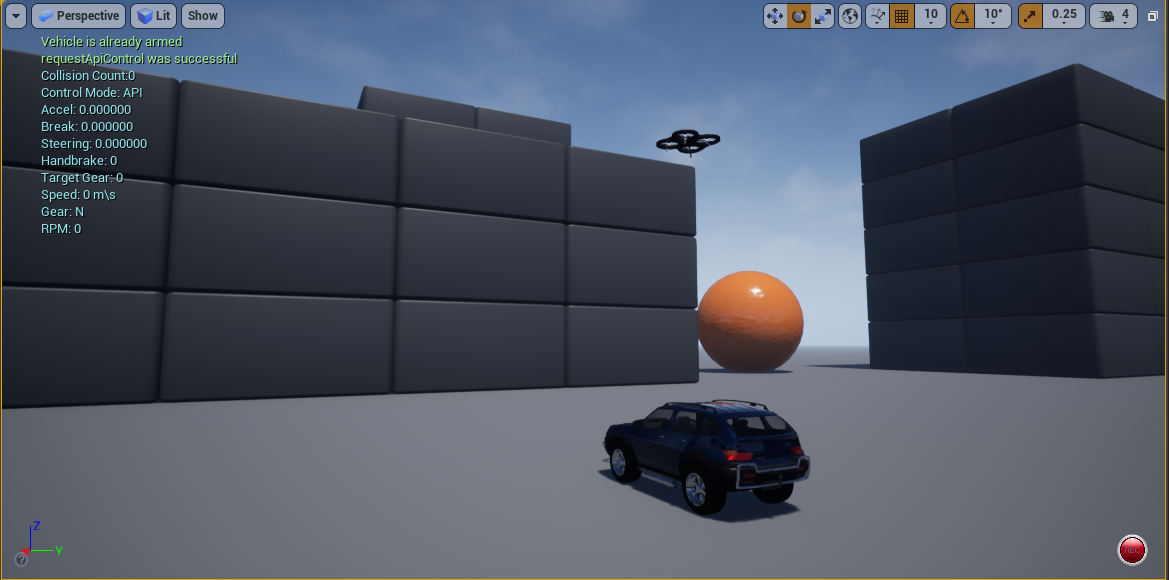
\includegraphics[width=.8\textwidth]{car_and_drone_1.png}
    \caption{Unreal Engine Block-world with drone and vehicle}
    \label{Block-world}
\end{figure}

We use the Microsoft Airsim simulator (based on UnrealEngine), allowing to simulate both a drone and a car, travelling in a 3D grid world (simulated as 3D blocks), while the drone control is given through a python script running in parallel receiving a feedback of the state parameters from the Airsim environment.
Roughly describing the problem flow, at each run we randomly initiate a goal and start position assuming the drone and car start together, have the drone path-plan a trajectory knowing the map of the world and execute it using our learned policy function while a human is controlling the vehicle thru the keyboard.
In the learning phase, during the run, the drone is rewarded per a set of metrics derived from its relative position w.r.t car (line-of-sight, relative orientation, distance, speed and time) and a terminal reward based on its overall success in the task (i.e., did it get to the goal together with the vehicle and how long it took it). 
Upon finishing an episode, the drone agent updates its policy-maker based on the experience it gained during the run (each experience being a tuple of state, action, reward and next state) and using an Actor-Critic RL scheme.
We also put significant work into the path-planning part, aiming to use a known planner but augment it to also incorporate a learned hyper-parameter controlling the smoothness of the trajectory. I.e., set for example a max$_$allowed$_$angle param controlling the chosen paths’ max turning angle. This parameter is also tuned by the system, though in a more conventional way, analyzing the true trajectory the drone and car drove along and tweaking the planning params if a big difference is observed. As a baseline,  we implemented both an augmented RRT planner (augmented to incorporate restraints on the allowed turning angle of the trajectory) and a PRM (Probabilistic RoadMap) method which we will go into more details later on.

We conducted overall approximately 3 hours of training (each episode taking an average of 100 seconds) and while this is not a lot of data in terms of learning algorithms, we were able to start seeing threads of learning, especially in the relation between relative distance and speed (i.e. action), pushing the drone to slow down if the vehicles is further away and vice-versa. We also saw similar linking between the relative speed and action and while maintaining the drones tendency to complete the path and not just stall in place (i.e. the time-penalty mechanism is working). Though much more data, especially in terms of diversity, is needed to conclude it a successful algorithm, we think it has the potential to learn even more complex relations and possibly in the future also derive its own state features for example based on on-board cameras. \

All our code (including setup instructions) could be found at: \\ 
\hyperlink{https://github.com/IdoMatan/RoboticGuidance}{https://github.com/IdoMatan/RoboticGuidance}


\section{Literature Review}

\paragraph{A Human-Robot Collaborative Reinforcement Learning Algorithm, \textit{Ali Shafti , Jonas Tjomsland , William Dudley and A. Aldo Faisal.}}  ~\cite{kartoun2010human}
A Soft-Actor-Critic RL algorithm implemented on the task of human-robot jointly controlling a tilting tray to direct a ball to a destination hole on the other end. The robot and human each control a different axis of rotation thus are forced to join-forces directing the ball to its destination. The user input is given through tilting a plate which translates (with a slight time-delay to further challenge both the human and robot) to a rotation angle of the game tray. The algorithm records the state of the tray and ball along with the human input as the state vector and accordingly derives a suitable action (i.e., the complementary rotation angle to the one the human instructed). The algorithm is tested against human-human interactions and proved half could reach the same level with one of the players being a robot (in terms of number of successful goal drops).

\newpage
\paragraph{The Interactive Museum Tour-Guide Robot,\textit{Wolfram Burgard, Armin B. Cremers, Dieter Fox, Dirk Hahnel, Gerhard Lakemeyery, Dirk Schulz, Walter Steiner, and Sebastian Thrun}} ~\cite{burgard1998interactive}
A robotic museum tour guide (named RHINO), able to navigate through a museum environment per a user’s request input on a given tour, cope with the rapidly changing environment and give added info on exhibitions. The robot leverages an impressive software stack (especially as it was done in 1998) to path plan (using a value iteration algorithm), update its, originally given, map accounting for moving humans and obstacles, and interact with the human both to initiate a tour and as its “instructor” of the tour. The robot successfully led over 2000 people touring the museum for a total of approximately 47 hours with minimal down time and while avoiding new and varying environments (daily moving of chairs, stools tables etc.) . In a sense, we aim to tackle a similar (and slightly simpler) task though focus on the optimization of completing the task (reaching the goal) while accounting for the human limitations thus focus more on human-maneuverability and limitation issues of human guidance.



\paragraph{Robot gains Social Intelligence through Multimodal Deep Reinforcement Learning, \textit{Ahmed Hussain Qureshi, Yutaka Nakamura, Yuichiro Yoshikawa and Hiroshi Ishiguro}} ~\cite{qureshi2016robot}
A human-robot interaction algorithm learning to interact with humans (specifically aiming to get a handshake) using camera and depth sensor inputs and leveraging a complete RL pipeline outputting one of 4 possible actions (wait, look for human, wave, attempt to shake hand). While this is slightly different from what we propose, it captures the algorithms’ need to adapt to different users (humans) each with a slightly different approach/skill. 



\paragraph{Deep Trail-Following Robotic Guide Dog in Pedestrian Environments for People who are Blind and Visually Impaired - Learning from Virtual and Real Worlds, \textit{Tzu-Kuan Chuang, Ni-Ching Lin , Jih-Shi Chen, Chen-Hao Hung, Yi-Wei Huang, Chunchih Teng, Haikun Huang, Lap-Fai Yu , Laura Giarre , and Hsueh-Cheng Wang}} ~\cite{chuang2018deep}
Design and implementation of a trail-following robot aiding the blind and visually impaired, the robot uses CNNs to detect the trail and follow it along leading the person using a rigid cane thus guiding it along the path. While the focus of the paper wasn’t on the user-experience side of guiding, they surveyed the participants after the trials and from our understanding there is room for the optimization of the interaction such that the users would get a reliable feel while adapting the speeds and maneuvers to the users (as some users of the above guidance dog felt it was slow at times and on other cases wanted a stronger interactions (possibly by pulling them harder of “nudging” them to follow). While the algorithm and focus of our work is slightly different than the above, the trials they performed and the general notion of robotic guidance is of value to our work.



\paragraph{AirSim: High-Fidelity Visual and Physical Simulation for Autonomous Vehicles, \textit{Shital Shah, Debadeepta Dey, Chris Lovet, Ashish Kapoor}} ~\cite{shah2018airsim}
The paper behind the simulator plugin we use to develop and test our algorithm. The plugin is the work of a team in Microsoft, built on top of the Unreal Engine (used to build computer games and much more) and enables the use of the Physical Engine, environmental rendering and more to develop algorithms in the field of drone and vehicle navigation and planning. The plugin enables both the remote controlling of a vehicle in the Unreal Engine simulator environment while also receiving feedback from simulator on current positions and velocities vectors to RGB and depth camera images, which could then be processed externally to generate new controls to be sent to the simulator. The plugging supports multiple scripting languages (we choose to work with Python) and is generally written in C++. The main strength of this is the use of realistic dynamic models of both vehicles and the environment (e.g. gravity, sun-light and much more) and the ability for rendered feedback creating almost realistic images for computer vision algorithms. Originally the simulator supported either drones or vehicles (not a combination of the two) but we augmented it slightly to allow support of both a drone and vehicle together for our specific use case in this project.

\paragraph{Reinforcement Planning: RL for Optimal Planners, \textit{Matt Zucker, J. Andrew Bagnell}} \cite{zucker2012reinforcement}
Implementation of an RL planner/controller able to capture/learn a more complex cost function than could be manually be written or demonstrated called Reinforcement Planner. The Idea behind the algorithm is to learn a value or policy mapping on-top of the cost-to-go (i.e. the distance to the goal for each state) which learns from experience the optimal action per a given state vector and thus subject to a more complex cost function then could have been manually ascribed. An experiment on a marble maze simulator was done (directing a marble on tilting frame with walls and holes from a start to goal pose) and proved the algorithm was able to learn over multiple trials a value function capturing the “dangerous” holes and the “safe” walls and able to achieve significantly better results the plain vanilla planning without the additional cost function.

\paragraph{Elaborating on Learned Demonstrations with Temporal Logic Specifications, \textit{Craig Innes, Subramanian Ramamoorthy}} \cite{innes2020elaborating}

Design and implementation of a more sophisticated method for learning from demonstrations usings Linear Temporal Logic constraints and the derivation of them as differentiable functions so they are able to serve as part of a loss/cost function of a planning/control problem. The main idea behind the paper is accompanying an expert demonstration with a logical constraint literal (i.e. a set of ground rules the robot has to abide to, such as “do this only after that”) thus implicitly giving him added insights/rules to the given task and reducing dramatically the amount of demonstrations needed. This is done using Linear Temporal Logic and more specifically a novel derivation of them as differentiable functions added to the loss function of the robot planner together with an adversarial method for learning the weights for a Dynamic Movement Primitive (DMP) generating robot trajectories. They implemented the above on a 2-D planar motion robot (a PR-2 robot) on a reach and cup pouring task which was able to learn and capture the constraints after only a few demonstrations while abiding the rules set by the LTL (such as don’t pour the cup before you are over the bucket). The above method is quite useful for problems such as the one we attempt to tackle where the data sources are limited while some of the basic “rules” or limitations could be quite easily elaborated by an expert. While our algorithm doesn’t learn from demonstrations we seek to possibly integrate a somewhat similar method (at least by some sense).

\paragraph{Model-Free Reinforcement Learning with Continuous Action in Practice, 
\textit{Thomas Degris, Patrick Pilarski, Richard Sutton}} \cite{degris2012model}
Proposing an extension to the model-free, policy gradient method to allow control of continuous systems and deriving an Actor-Critic algorithm with eligibility traces for such problems. The use of eligibility traces together with the policy-gradient method allows for a feasible backward-view scheme and proved to work on several experiments they conducted on the Mountain-Car, pendulum and a moving  robot, allowing them to both converge quicker then compared algorithms as well as adapt to a varying scenario (specifically with the mobile robot running it both with the wheels lifted up and touching the ground). The base of this AC algorithm lays in the use of adding to the loss function of the actor and the critic terms simultaneously learning the value function of the game and thus augmenting the actor gradients wrt relevant errors per the given state (reducing variance significantly). 

\paragraph{Clear and smooth path planning, \textit{Mansoor Davoodi, Fatemeh Panahi, Ali Mohades, Seyed Naser Hashemi}} \cite{davoodi2015clear}
A derivation of two multi-objective problem propositions for path planning with added constraints such as energy consumption (also referred often as smoothness), obstacle avoidance, distance (or weighted distance) and more. The authors augmented the objective function operators accounting for the new constraints and formulated the problems such that solving them would derive an optimal (in the sense they describe) path. They also implemented a genetic algorithm with the above which proved to indeed derive paths confined to their constraints both in sparse and dense maps. In our augmentation of the loss functions of the path planners we used  their turning-angle cost to reward/penalize our planner and to also push towards smooth paths (in aim to have the drone agent limit its turning angle wrt how well the human car player managed to follow him in the previous sessions).

\paragraph{Rapidly-Exploring Random Trees - A new tool for path planning, \textit{Steven M. LaValle}} \cite{lavalle1998rapidly} - The original implementation of RRTs, an multi-dimensional path planning algorithm based on randomly evolving trees, creating, fast, yet not necessarily optimal paths given an obstacle space, start and goal. The idea behind the algorithm is having trees randomly evolve in the free-space (the n-dimensional space the robot is “allowed” to live in) until reaching the terminal state while accounting for the obstacles and the dynamics of the agent. As said earlier, while this does not guarantee an optimal path (i.e. in terms of distance), it creates it very quickly compared to other path planning algorithms such as PRM or others. Furthermore, this sort of planning also allows planning for non-holonomic agents (i.e. a car) as it can incorporate dynamic models and constraints in the “choosing” of next branches in the tree. The algorithm is tested on various test cases showing promising results in solving collision-free dynamic planning with constrained vehicles in multi-dimensional obstacle spaces.


\newpage
\section{Methods}
\paragraph{Main Framework} Built  with Python using the AirSim plugin. The interaction with the simulator (as can be seen in diagram 1) is initially to get a map of the world, done by sending the drone to a high altitude and snapping a bird's-eye view of the world, then, after a path in planned, to execute it sequentially (it is broken down to sub-segments where each is a mile-stone) while the human player tries to follow the drone. In parallel, a state vector consisting of attributes derived from both the drone and vehicle locations is drawn and saved for both the calculation of next action, i.e. if and at what speed continue to fly and for later to learn the path planning hyper-parameters as will be described later. 

\begin{figure}[!h]
    \centering
    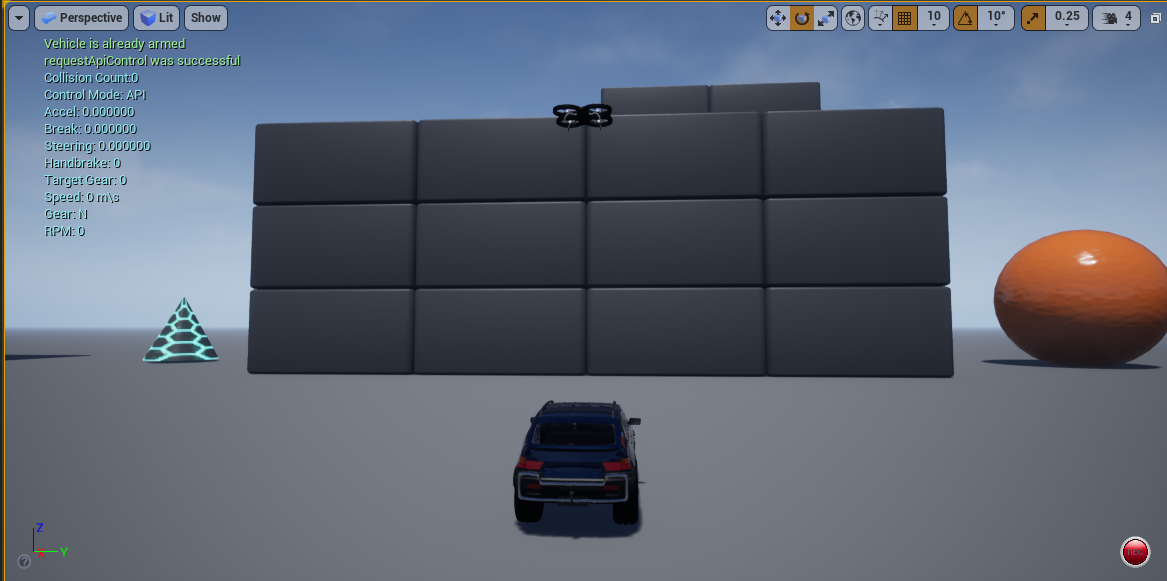
\includegraphics[width=.8\textwidth]{drone_car_2.png}
    \caption{The Unreal-Engine simulator set up with a vehicle and drone together in the blocks-world environment. This is the starting pose of the game and from there the drone has to fly to the goal and the vehicle controlled by a human (thru the keyboard) has to follow him there}
    \label{fig:simulator}
\end{figure}

\paragraph{Path Planning} - We implemented two methods, both run on the acquired map from the simulator and a random initial and goal positions.


\begin{enumerate}
\item{\textbf{Smooth RRT}} - A flavour of the Rapidly-Exploring Random Trees with the addition of limiting the allowed turning angle of a given path. The algorithm is similar to the original one only upon checking whether a new branch is feasible (i.e. in terms of obstacle avoidance) we added a max turning angle threshold check looking at the previous node and calculating the needed turning angle between the two edges and only allowing ones benether the TH. This hyperparameter is flexible and will be controlled/learnt by the algorithm per the experience it gained from previous episodes. While this does not necessarily derive an optimal path, as it runs quickly in a sparse environment, we were able to perform several runs, each generating a trajectory together with a cost and then choose the best one.

\begin{figure}[!h]
    \centering
    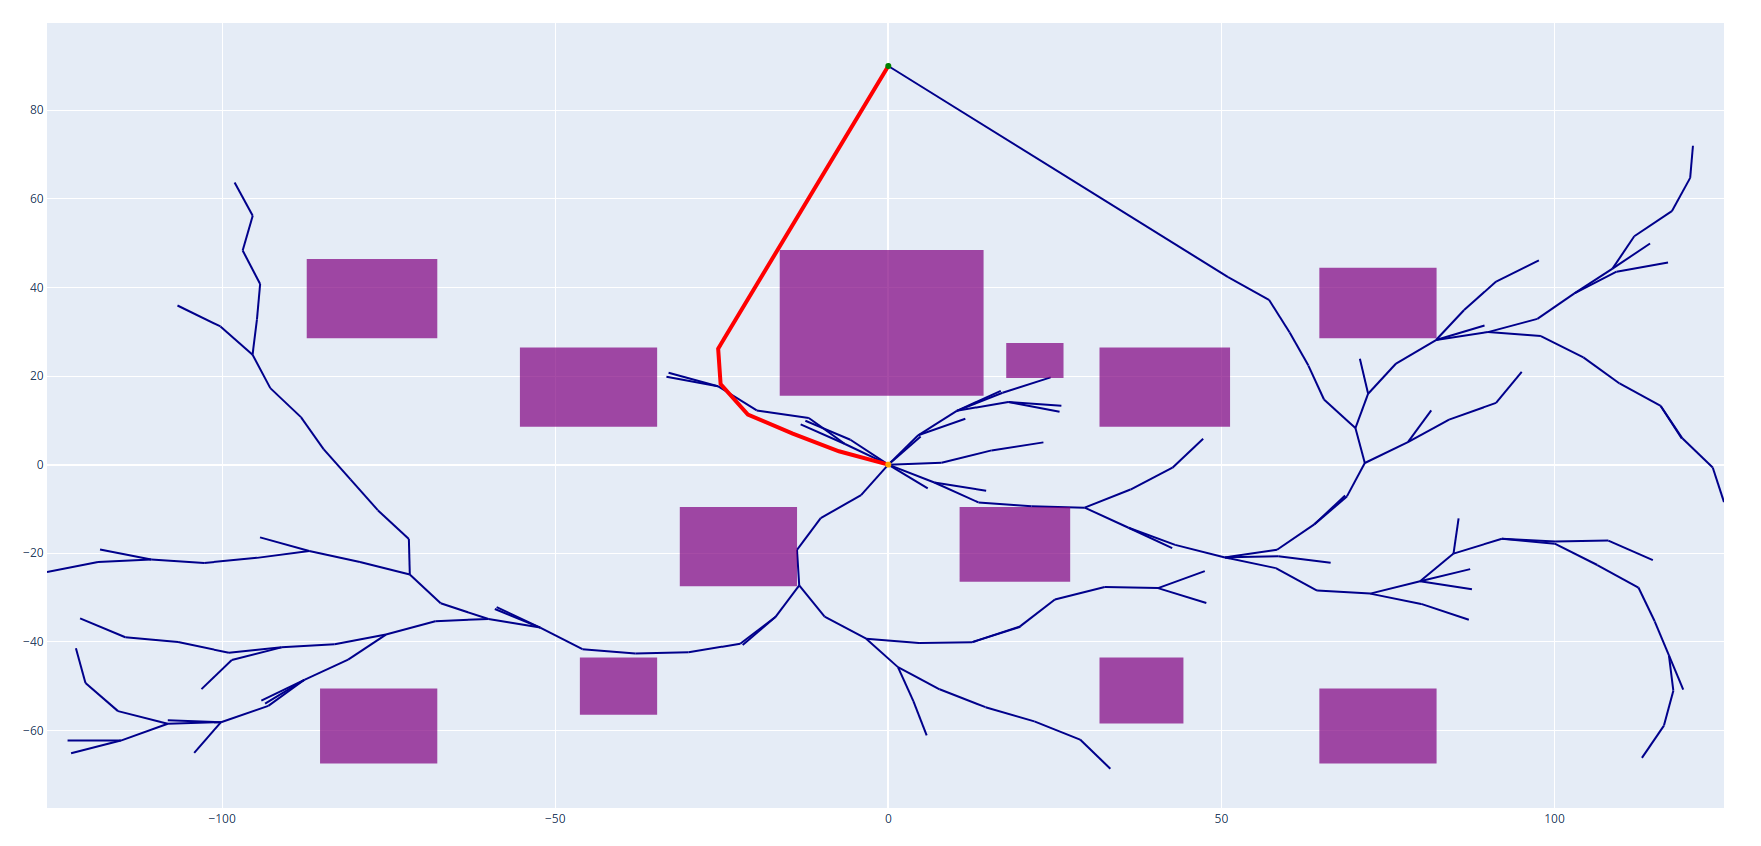
\includegraphics[width=.6\textwidth]{RRT.png}
    \caption{Path found by the smooth-RRT algorithm, as can be seen only branches inducing a turning angle of less than 50degrees were allowed thus a smooth path was derived.}
    \label{fig:RRT}
\end{figure}

\newpage
\item{\textbf{PRM with BFS}} -like Dynamic Programming planner designed to find an optimal path from the start to goal, but wrt both the distance and smoothness of the path. To do so each node has to keep not only the shortest path to it but also the smoothness of traversing from each of its neighbors so that if reached from a new node it could re-calculate what best path would fit from there on. The cost weight of turning compared to distance is controllable and could be adjusted by the algorithm. While in theory the algorithm should derive an optimal path (in the sense described above and wrt to the graph the PRM generated), the complexity of it sometimes is not worth the time compared to the RRT algorithm which in less dense environments converges rather quickly.\
\end{enumerate}

\begin{figure}[h]
    \centering
    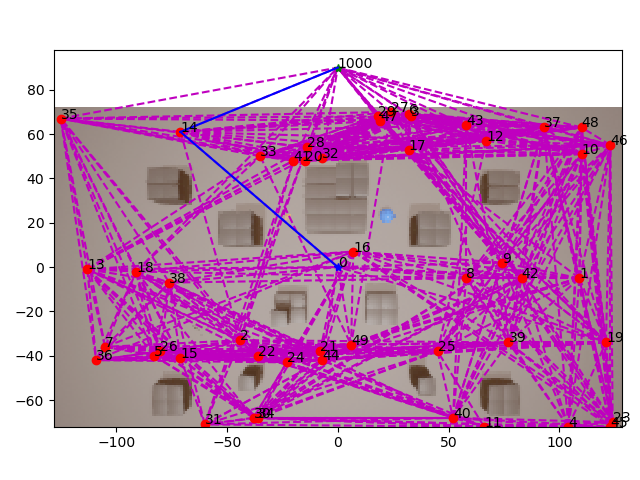
\includegraphics[width=.6\textwidth]{prm.png}
    \caption{Path found by the smooth PRM-like algorithm. Note the path is only optimal wrt points it randomly generated (thus globally optimal only if number of points tends to infinity)}
    \label{fig:PRM}
\end{figure}

After testing both, we decided to continue with the RRT based method for the implementation of the algorithm, mainly due to its sufficient results in the simplified environment and the overall running time of each episode. That said, if need be, both (or any other planning heuristic) could be plugged in and used as a path planning block.



\paragraph{Execution block} In charge of communicating with the simulator, both to send the next action (‘Fly to \texttt{\char`_} at \texttt{\char`_} m/s’) and log the state vectors from the simulator. Our current state vector consists of: {distance between drone and car, line of sight, relative heading angle,  relative speed, drone speed}. The execution block also calculates the next action based on the state vector and sends the drone an action, currently from the options pool of: {‘Fly to $__$ at $__$ m/s’, wait in place}.



\paragraph{Train Cycle} Following a complete episode (a full run together with a human player) the experience log is used to update the policy maker (the block in charge of deciding on an action per a given state as described in the execution block and setting the max allowed angle for the planning algorithm). This is done as with other RL algorithms using the Bellman Error, i.e., what we expected the value of the next state to be compared to what it turned out to actually be.
After finishing the episode we calculate the average relative pose between the car and the drone along the epoch to update the path planner smoothness TH according to how well the car and drone trajectories we're consistent (i.e. the car managed to accurately follow the drone). We do so in a simple control loop increasing or decreasing the maximum turning angle allowed by the planner w.r.t episode results described above.\\
\\A pseudo code version of the algorithm is:\\


\begin{algorithm}[H]
\SetAlgoLined
\DontPrintSemicolon % Some LaTeX compilers require you to use \dontprintsemicolon instead
\KwIn{AirSim env, player}
\KwOut{Actor and critic trained models and path planner smoothness TH}
\vspace{1.5mm}
\For {each episode (game with human)}{
Initialize randomly start and goal\;
Get map and plan path for drone (goal is hidden from human player)\;
\While{not at goal state (and at a $1Hz$ loop):}{
Get current state vector from simulator\;
Calc reward and speed/action based on current state vector\;
Send to drone new action\;
Log state-action-reward-next$_$state\;
\If {reached goal or time is up}{Break}

}
Update policy function wrt experiences logged in episode\;
Update planner params wrt experiences logged in episode\;

}
\Return{Actor and critic models}\; \label{algl2:l4}
\caption{Agent training}
\label{algo:training}
\end{algorithm}


\newpage
\paragraph{Algorithm - Policy Maker block} we implemented an RL algorithm with an Actor-Critic scheme, i.e. 2 different neural networks, one outputting a probability distribution over the possible actions (a discrete representation of speeds from 1 to 10) and the second the value\footnote{The value of the state being an known RL term for how good the state is in terms of the final goal of the game, i.e. being a meter away from the goal and without and obstructions in the way would have a higher value than an intermediate state without any line-of-sight to the goal (loosely speaking).
} of the specific state, the first is used to generate the next action and the second to reduce the variance of the loss term in the learning process. We won’t go into all the details of the working mechanics of the RL algorithm as it's a known scheme and not our novel work. Our implementation consisted of implementing it so it receives the state vector we extract from the simulator in real-time and return the action to the simulator to execute. A lot of effort also went into the reward shaping of the algorithm, i.e., on what the agent gets rewarded/penalized for and moreover at what scale. Currently, the agent will get a time-penalty of -1 every second (to generate a tendency to complete the path), a -50 penalty if there is no line-of-sight between the agents, a penalty on relative distance, speed and heading of the drone and car and a milestone reward for reaching nodes in the planned trajectory graph (also to generate an incentive to complete the path). We played with the scale of the parameters balancing the tendency to complete the path vs. “politeness” and we think further work could be done to generate more rewarding heuristics to generate more optimal policy makers.


\begin{figure}[h]
    \centering
    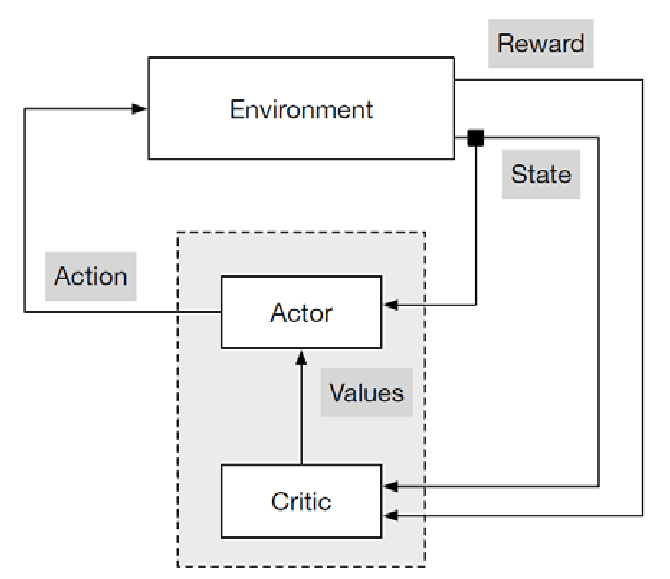
\includegraphics[width=.5\textwidth]{A2C.png}
    \caption{a general Actor-Critic scheme taken from Elmar Diederichs’ “Reinforcement Learning - A Technical Introduction”}
    \label{fig:A2C}
\end{figure} 



\newpage
\paragraph{Architecture} In figure ~\ref{fig:Architecture} a block diagram describing the process as we implemented it can be found to further clarify the working scheme 

\begin{figure}[!h]
    \centering
    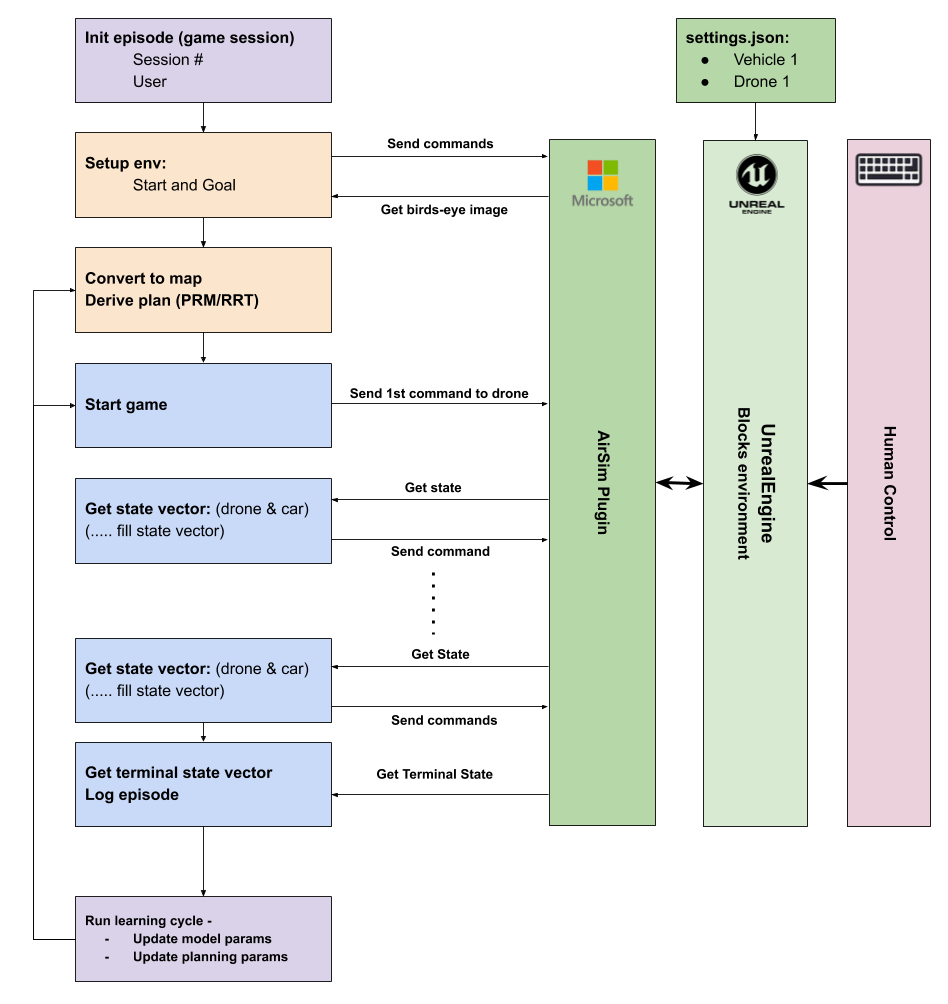
\includegraphics[width=.7\textwidth]{GuidanceDrone_Architecture.png}
    \caption{A schematic block diagram of the training mechanism}
    \label{fig:Architecture}
\end{figure}




\section{Results}

To train our agent we had overall approximately 100 training episodes (games), each training episode took about 100 seconds (until either reaching the goal or timing out). The training was done by 3 different users and tested by 7 users, each playing 10 evaluation games.

In graph ~\ref{fig:reward} the average reward of each episode during the learning phase can be seen. As could be noticed, at around 40-50 episodes the algorithm was able to capture the relation between the penalty of relative distance and started to slow down when the car was further away. That said, all the episodes were also finished within 100 seconds or less (thus it kept pursuing its goal reward). \\


\begin{figure}[h]
    \centering
    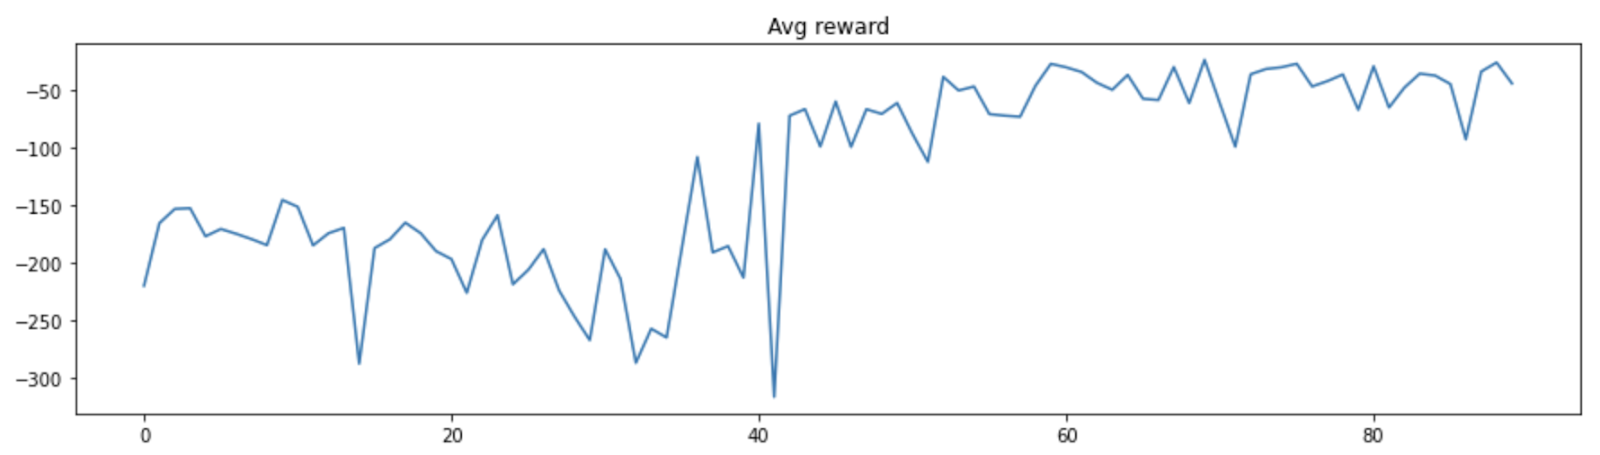
\includegraphics[width=.9\textwidth]{reward.png}
    \caption{Average reward on last 90 episodes (games). After about 40 episodes the drone “learned” it's better to wait for the car to reduce the relative distance penalty.}
    \label{fig:reward}
\end{figure}

\newpage
In figure ~\ref{fig:Epoch}, we plotted the action-relative distance relation in one epoch. As can bee seen, one of the first things the agent learned was to slow down when the relative distance increased (i.e. the car was far behind the drone). 

\begin{figure}[h]
    \centering
    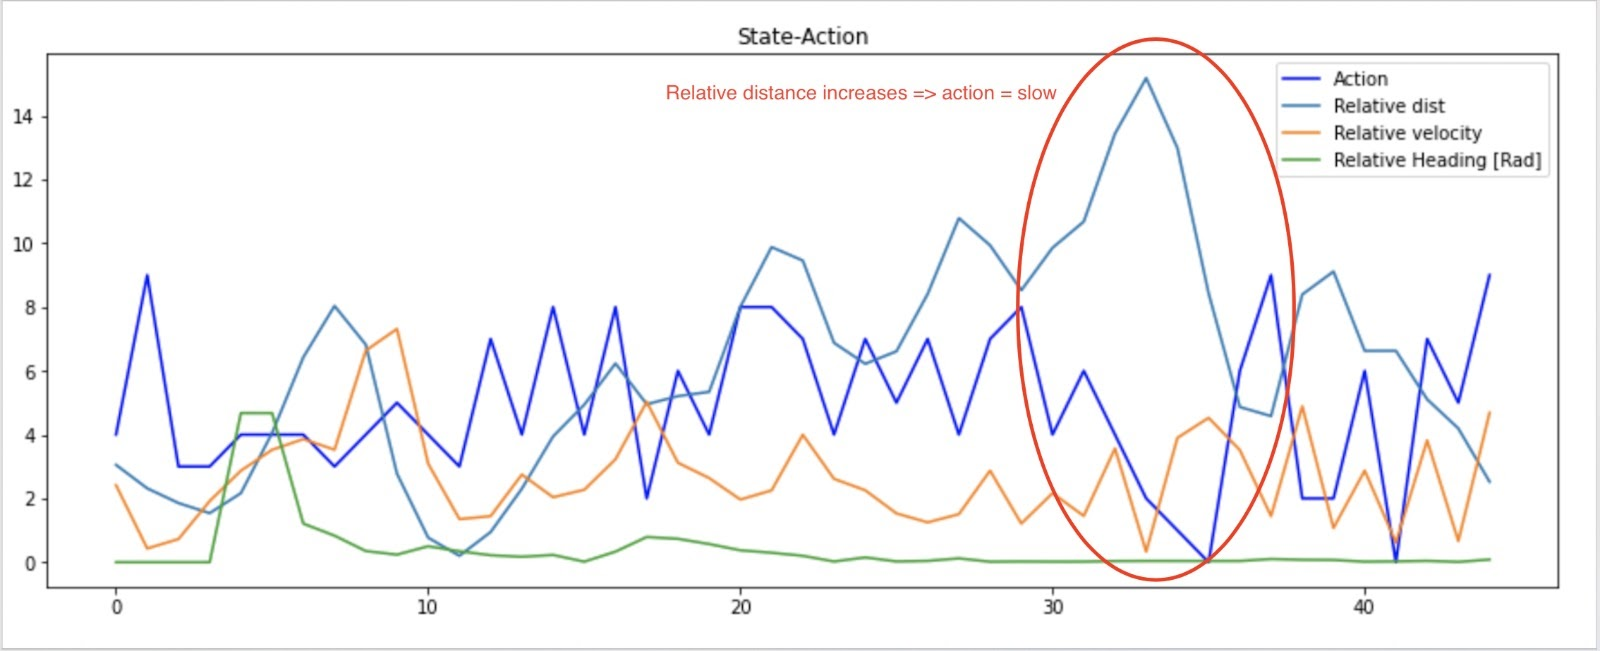
\includegraphics[width=.8\textwidth]{epoch.jpeg}
    \caption{state-action plot, as can be seen after approximately 60 runs the drone “learned” to slow down when the car was further away}
    \label{fig:Epoch}
\end{figure}

In table \ref{tbl:tests} we've summarized the tests results of 7 different users, each playing 10 games and with some having prior experience (i.e. played the game before) while others played for the first time. As can be seen, achieving an average result of 80\% success rate (i.e., both the drone and car reached the goal within a reasonable lag).

A second order observation is the general speed reduction, most likely to satisfy the penalty/reward for relative speed. Having said the above, as can be seen in table \ref{tbl:tests}, a user with only 2 ‘introduction’ games, was able to complete the game for 8/10 games and get an overall success rate of ~80\%.\\


\begin{table}[ht]
\begin{center}
\caption{Summary of test runs on 7 different users}
\label{tbl:tests} 
\begin{tabular}{|c|c|c|c|c|} 
\hline

User & Experience (pre-runs) & Test Games & Score & Success rate \\
\hline
01 & 64 (agent train) & 10 & 9 &  90\%    \\ 
02 & 47 (agent train) & 10 & 9 &  90\%    \\
03 & 5                & 10 & 7 &  70\%    \\
04 & 10 (agent train) & 10 & 7 &  70\%    \\ 
05 & 4                & 10 & 8 &  80\%    \\
06 & 2                & 8  & 7 &  87.5\%  \\ 
07 & 0                & 8  & 6 &  75\%    \\

\hline

\multicolumn{1}{|c|}{Overall} & \multicolumn{3}{c|}{ } & \multicolumn{1}{c|}{80.1\%} \\
\hline
\end{tabular}
\end{center}
\end{table}


Nevertheless, there is still much more training needed to actually optimize the algorithm and have it trained on a more diverse dataset (i.e. more users) to reduce the bias of us learning to play and to allow it to capture more complex insights on the human agent.

while much more data is needed to conclude the algorithm is indeed working and more specifically testing it with more new users, the results as can be seen, do indicate learning is taking place) 


\section{Discussion}
Our main takings from this project are first of all the complexity of actually setting up an environment for such algorithms to be built and trained, and more specifically the work with the external simulator and plugins we had to set up. Furthermore, the challenge of gathering data where each episode has to be done together with a human (as opposed to an algorithm learning to play a video game for example) is a great challenge in algorithms needing a mass amount of training data to converge and thus in some cases a reduction in complexity or a breakdown to sub-problems is needed to actually allow learning to be feasible. That said, we were excited to actually see the drone start to capture the (though trivial) constraints of human/car response time and the speed limitations, and do believe that with further work and training data it could get even further.
With more time available, we would first invest some more time on stabilizing the platform and replicating it so we could have it train asynchronously and thus enlarge our training set. Second, explore the state vector structure and content, initially to include more broad metrics of the state and later to possibly even feed it with just a camera input from the drone and have its neural network learn to extract the states features by itself (a romantic idea though requiring a massive amount of data). Furthermore, shaping of the reward function could definitely yield improvement, both scaling it appropriately and finding more sophisticated mechanics to base on.
Our initial intentions on this project were algorithms able to capture human constraints towards robots cooperating and specifically guiding people in various environments, at this stage we think we capture the complexity of designing such algorithms yet are optimistic that with careful reward shaping and trying to keep things simple and even slightly fragmented it's possible to do and to be honest very interesting and would be even more so with future integration of actual robots.


\section{Appendix} All our code (including instructions on how to set things up) can be found here:\\ \hyperlink{https://github.com/IdoMatan/RoboticGuidance}{https://github.com/IdoMatan/RoboticGuidance}




\bibliographystyle{ieeetr}
\bibliography{main}

%++++++++++++++++++++++++++++++++++++++++


% \begin{thebibliography}{99}


% \end{thebibliography}


\end{document}
